%----------------------------------------------------------------------------------------
%	PACKAGES AND DOCUMENT CONFIGURATIONS
%----------------------------------------------------------------------------------------

\documentclass{article}

\usepackage[version=3]{mhchem} % Package for chemical equation typesetting
\usepackage{siunitx} % Provides the \SI{}{} and \si{} command for typesetting SI units
\usepackage{graphicx} % Required for the inclusion of images
\usepackage{natbib} % Required to change bibliography style to APA
\usepackage{amsmath} % Required for some math elements 
\usepackage{placeins}
\usepackage[font=small,labelsep=space]{caption}
\captionsetup{%
  figurename=Fig.,
  tablename=Table
}
\setcitestyle{square}
\setlength\parindent{0pt} % Removes all indentation from paragraphs

\renewcommand{\eqref}[1]{\textup{{\normalfont(\ref{#1}}\normalfont)}}

\renewcommand{\labelenumi}{\alph{enumi}.} % Make numbering in the enumerate environment by letter rather than number (e.g. section 6)

%\usepackage{times} % Uncomment to use the Times New Roman font

\textheight=8.5in
\topmargin=-0.5in

%----------------------------------------------------------------------------------------
%	DOCUMENT INFORMATION
%----------------------------------------------------------------------------------------

\title{Homework 1} % Title

\author{Kenneth \textsc{Chaney}} % Author name

\date{\today} % Date for the report

\begin{document}

\maketitle % Insert the title, author and date

\begin{center}
\begin{tabular}{l r}
Date Performed: & November \(13^{th}\), 2014 \\ % Date the experiment was performed
Instructor: & Professor Dandekar \\ % Instructor/supervisor
Class: & ECET-512
\end{tabular}
\end{center}

% If you wish to include an abstract, uncomment the lines below
\begin{abstract}
The goal of this homework is to simulate a single user traveling through a cellular network while using new path loss equations in Part A. The co-channel interference (CCI) is also observed within this cellular network in Part B. Finally the signal to interference ratio (SIR) is analyzed in Part C.

\end{abstract}

\pagebreak
%----------------------------------------------------------------------------------------
%	SECTION 1
%----------------------------------------------------------------------------------------

\section{Part A}\label{partA}

To generate results for this section run the demoA.m file. The animation generated shows the mobile user traveling accross each cell. After the animation is complete a graph showing signal strength vs frame number is generated as shown in figure \ref{parta}. \\ 

The path loss model used is shown in equation \ref{pathloss}. The shadowing is modeled by the random variable \( \epsilon \). Each \( \beta \) tested has a central mean for the trajectory followed and the shadowing applies a variation from that central meani--as can be seen in figure \ref{parta}. Each time the test is run the shadowing will be slightly different while the mean will stay approximately the same (there is a possibility for the randomness to be skewed in one direction). \\

\begin{equation}\label{pathloss}
P_r(d)=E\begin{bmatrix}P_r(d_0)\end{bmatrix}-10\beta log_{10}\dfrac{d}{d_0}+\epsilon
\end{equation}

\begin{figure}[h]
\centerline{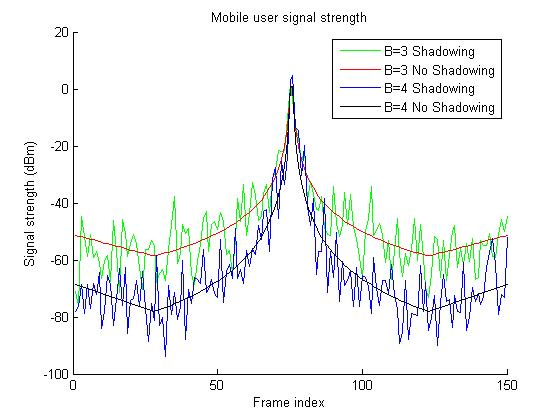
\includegraphics[width=5in]{latex/images/PARTA.jpg}}
\caption{Signal strength of recieving cell with new path loss equation.}
\label{parta}
\end{figure}

\clearpage

\section{Part B}\label{partB}

To generate results for this section run the demoB.m file. A similar animation to Part A will show up and a graph will appear at the end. However a video of the animation will be generated. The graph at the end is shown in figure \ref{partb}. \\

The path loss model is used to generate the loss in CCI. There are two \( \beta \) values that were calculated and each was shown with and without shadowing effects. The representations of no shadowing effects should approximately be the mean of the graph with the shadowing effects. The effect of the higher \( \beta \) is that there is more loss in the signal over the long distances that it must travel to cause CCI. \\

\begin{figure}[h]
\centerline{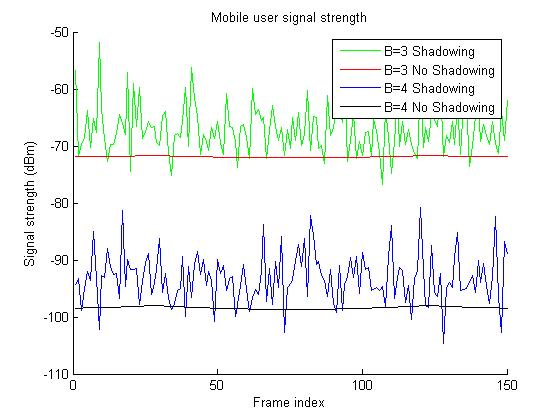
\includegraphics[width=5in]{latex/images/PARTB.jpg}}
\caption{CCI observed by the mobile user.}
\label{partb}
\end{figure}


\clearpage

\section{Part C}\label{partC}

To generate results for this section run the demoC.m file. A similar animation to Part A will show up and a graph for each \(\beta\) will appear at the end--similar to those in figures \ref{N3B3}-\ref{N7B4}. Each graph contains a SIR curve with shadowing, SIR curve without shadowing, SIR edge estimation, and SIR center estimation. The estimations were bounding the lower ranges on each of the graphs giving a good worst case scenario given the path loss model that was being used. \\

In general as N and \( \beta \) increased the SIR became more favorable. This is important to understand for a link budget because there is a better signal within a given cell as the number of channel bands you have increases and as your \( \beta \) increases. This makes sence because the interference will have more distance to dissipate while the actual signal still remains relatively strong.

\begin{figure}[h]
\centerline{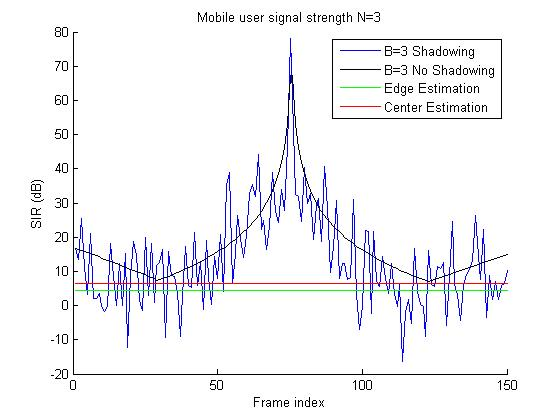
\includegraphics[width=5in]{latex/images/N3B3.jpg}}
\caption{SIR at mobile user location with N=3 and beta=3.}
\label{N3B3}
\end{figure}

\begin{figure}[h]
\centerline{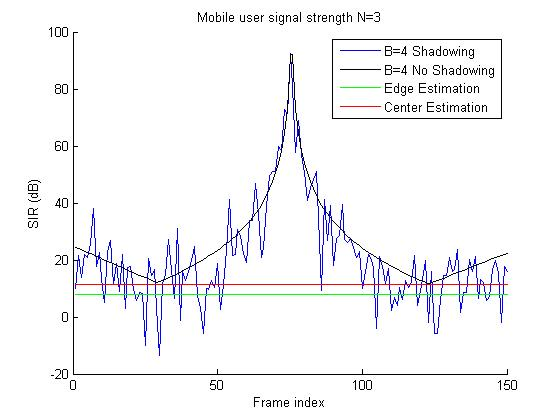
\includegraphics[width=5in]{latex/images/N3B4.jpg}}
\caption{SIR at mobile user location with N=3 and beta=4.}
\label{N3B4}
\end{figure}

\begin{figure}[h]
\centerline{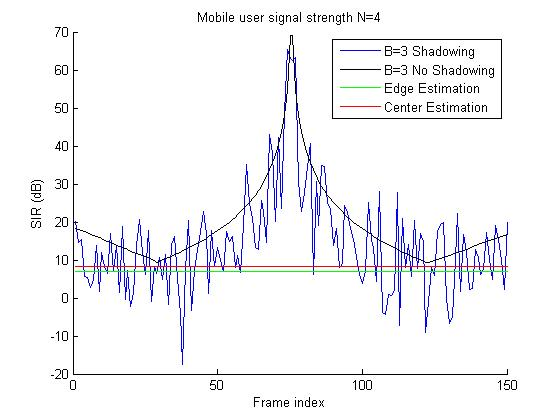
\includegraphics[width=5in]{latex/images/N4B3.jpg}}
\caption{SIR at mobile user location with N=4 and beta=3.}
\label{N4B3}
\end{figure}

\begin{figure}[h]
\centerline{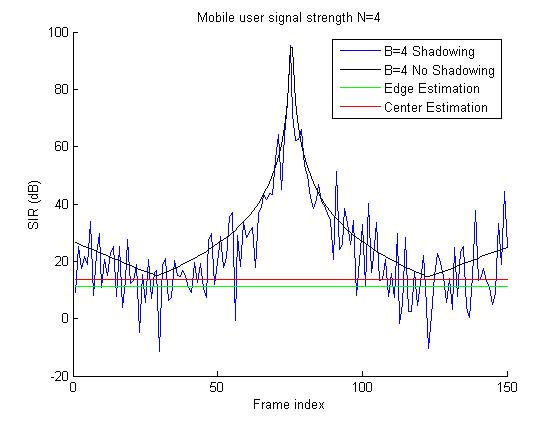
\includegraphics[width=5in]{latex/images/N4B4.jpg}}
\caption{SIR at mobile user location with N=4 and beta=4.}
\label{N4B4}
\end{figure}

\begin{figure}[h]
\centerline{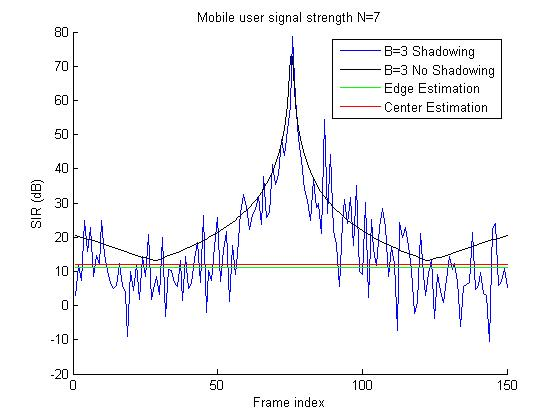
\includegraphics[width=5in]{latex/images/N7B3.jpg}}
\caption{SIR at mobile user location with N=7 and beta=3.}
\label{N7B3}
\end{figure}

\begin{figure}[h]
\centerline{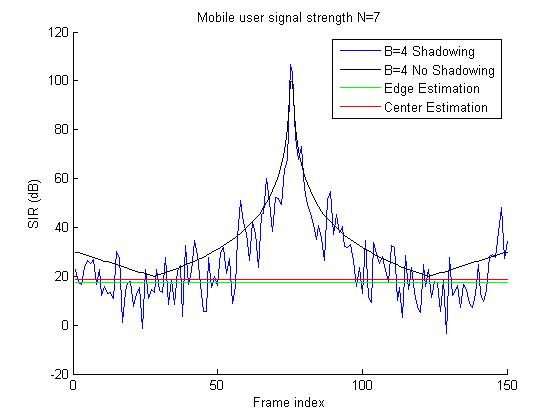
\includegraphics[width=5in]{latex/images/N7B4.jpg}}
\caption{SIR at mobile user location with N=7 and beta=4.}
\label{N7B4}
\end{figure}


\end{document}
